\section{Questions sur le chapitre ``La thermodynamique des vapeurs''}
\subsection{Donnez les définitions du point critique et du point triple d'une substance. Quel est le nombre de degré de liberté d'une substance au point triple ?}
\begin{description}
\item[Point critique] : le point critique $K$ est le point dans le diagramme ($p$,$v$) d'un fluide vaporisable (Fig. \ref{fig:diag_vdw}) où il n'y a plus de variation de volume lors d'un changement de phase. L'isotherme critique $T_K$ présente un point d'inflexion à tangente horizontale au point $K$. Au-delà de cette température, la seule phase possible est la phase gazeuse.
\item[Point triple] : le point triple $TR$ est le point dans le diagramme ($p$,$T$) d'une substance pure en lequel coexistent les trois phases solide, liquide et gazeuse.
\end{description}
\textbf{La règle des phases de Gibbs} établit une relation entre 
\begin{itemize}
\item $\psi$, le nombre de variables indépendantes intensives déterminant l'état d'un système thermodynamique en équilibre. Ces variables sont aussi appelées degrés de liberté du système;
\item $r$, le nombre de phases;
\item $n$, le nombre de constituants du système.
\end{itemize}
La règle des phases s'exprime par la relation suivante :
\begin{equation} \psi = n - r + 2 \end{equation}
La règle des phases joue un rôle particulièrement important en thermodynamique chimique. Dans le cas d'une substance pure ($n=1$), la règle des phases s'écrit plus simplement :
\begin{equation} \psi = 3 - r \end{equation}
Il en résulte que, pour les substances pures dans un système à une seule phase ($r=1$), le nombre de degrés de liberté est égal à 2. Ces variables indépendantes peuvent être la pression et la température par exemple. 

Au point triple, en $TR$, on a $r=3$, d'où $\psi = 0$. Il n'y a donc aucun degré de liberté lorsque l'on veut atteindre la coexistence des trois phases : un état et un seul est possible en ce point.

\begin{figure}[p]\centering
	\tikzsetnextfilename{diagramme_pv_vdw}
    \begin{tikzpicture}
        \begin{axis}[
        	enlargelimits=true,
        	grid=major,
        	axis lines=left, xtick=\empty, ytick=\empty,
        	xmin = 0.1, xmax = 3.6,
        	ymin = 0.2, ymax = 1.6,
        	ylabel=$p$,
        	xlabel=$v$,
		]
			\addplot [green] table[col sep=comma] {data/vdw1.csv} node[right ,pos=1]{\small$T > T_K$};
			\addplot [green] table[col sep=comma] {data/vdw2.csv};
			\addplot [green] table[col sep=comma] {data/vdw3.csv};
			\addplot [green] table[col sep=comma] {data/vdw4.csv};
			\addplot [red] table[col sep=comma] {data/vdw5.csv} node[right ,pos=1]{\small$T = T_K$};
			\addplot [blue] table[col sep=comma] {data/vdw7.csv};
			\addplot [blue,dashed] table[col sep=comma] {data/vdw8.csv};
			\addplot [blue] table[col sep=comma] {data/vdw9.csv};
			\addplot [blue,dashed] table[col sep=comma] {data/vdw10.csv} node[right ,pos=1]{\small$T < T_K$};
			\addplot [black,thick] table[col sep=comma] {data/vdw6.csv} node[below, pos=0]{\footnotesize Ébullition} node[below,pos=1]{\footnotesize Rosée};
			\draw (1,1) node{$\circ$} node[above]{\small$K$};
			\draw (0.3,0.75) node[fill=white,draw,rectangle]{\small$L$};
			\draw (1.3,0.5) node[fill=white,draw,rectangle]{\small$L+V$};
			\draw (2.7,0.65) node[fill=white,draw,rectangle]{\small$V$};
			\draw (2.5,1.2) node[fill=white,draw,rectangle]{\small$G$};
        \end{axis}
    \end{tikzpicture}
    \caption{Diagramme ($p$,$v$) d'un fluide vaporisable}
    \label{fig:diag_vdw}
\end{figure}
\begin{figure}[p]\centering
	\tikzsetnextfilename{diagramme_phase}
    \begin{tikzpicture}
        \begin{axis}[
        	enlargelimits=true,
        	grid=major,
        	axis lines=left, xtick=\empty, ytick=\empty,
        	xmin = 180, xmax = 310,
        	ymin = -0.2, ymax = 2,
        	ylabel=$p\;(\si{\bar})$,
        	xlabel=$T\;(\si{\kelvin})$,
		]
            \addplot [blue,domain=194.4:216.58,samples=200] {ln(9700000*exp(-26000/(8.314*x)))/ln(10)} node[pos=1]{$\circ$} node[below right, pos=1] {$TR$};
            \addplot [blue,domain=216.6:304.2,samples=200] {ln(0.0000377*x^3 - 0.0217*x^2 + 4.338*x - 299.384)/ln(10)} node[pos=1]{$\circ$} node[right,pos=1]{$K$};
            \addplot [blue,domain=216.1:350,samples=200] {ln(13500*exp(-400/(8.314*(x-210))))/ln(10)};
            \draw (200,1) node[fill=white,draw,rectangle]{\small$S$};
			\draw (260,0.5) node[fill=white,draw,rectangle]{\small$G$};
			\draw (240,1.5) node[fill=white,draw,rectangle]{\small$L$};
        \end{axis}
    \end{tikzpicture}
    \caption{Diagramme ($p$,$T$) d'une substance pure}
    \label{fig:diag_phase}
\end{figure}

\subsection{L'équation d'état de van der Waals est donnée par \ref{eq:vdw}. Expliquez la signification physique des constantes $a$ et $b$ et comment on les obtient à partir des variables d'état au point critique.}
En se basant sur des considérations très simples de théorie cinétique des gaz, van der Waals a proposé l'équation d'état à deux constantes :
\begin{equation} p = \frac{RT}{v-b} - \frac{a}{v^2} \label{eq:vdw} \end{equation}
avec $a$ la force d'attraction intermoléculaire et $b$ le covolume lié au volume propre des molécules, qui n'est négligeable par rapport au volume total que si la pression est faible.  

On calcule ces constantes par l'existence d'un point d'inflexion à tangente horizontale en $K$ pour l'isotherme critique dans un diagramme ($p$,$v$) (Figure \ref{fig:diag_vdw}) : 
\begin{equation} \left.\fpart{p}{v}\right|_{T_K} = 0 \qquad \text{et} \qquad \left.\ffpart{p}{v}\right|_{T_K} = 0 \end{equation}
On réécrit ces conditions sous la forme :
\begin{align} \left.\fpart{p}{v}\right|_{T_K} &= -\frac{RT_K}{(v_K - b)^2} + \frac{2a}{v^3_K} = 0 \\ \left.\ffpart{p}{v}\right|_{T_K} &= \frac{2RT_K}{(v_K - b)^3} - \frac{6a}{v^4_K} = 0 \end{align}
On en déduit :
\begin{equation} v_K = 3b \qquad \text{et} \qquad T_K = \frac{8a}{27Rb} \end{equation}
et l'on trouve par l'équation d'état :
\begin{equation} p_K = \frac{a}{27b^2} \end{equation}

\subsection{Démontrez qu'au point critique la relation \ref{eq:crit} est valable pour un gaz si l'on suit l'équation d'état de van der Waals.}
\begin{equation} \left(\fpart{T}{v}\right)_{p_K} = 0 \label{eq:crit} \end{equation}
Selon l'équation d'état de van der Waals, la température s'exprime de la manière suivante :
\begin{equation} T = \left(p + \frac{a}{v^2}\right)\frac{(v-b)}{R} \end{equation}
On dérive ensuite cette équation :
\begin{equation} \left(\fpart{T}{v}\right)_{p_K} = \left(p_K + \frac{a}{v^2_K}\right)\frac{1}{R} + \left(\frac{v_K-b}{R}\right)\frac{-2a}{v^3_K} \end{equation}
Or au point critique :
\begin{equation} v_K = 3b \qquad \text{et} \qquad p_K = \frac{a}{27b^2} \end{equation}
Et donc :
\begin{align} \left(\fpart{T}{v}\right)_{p_K} &= \left(\frac{a}{27b^2} + \frac{a}{9b^2}\right)\frac{1}{R} + \frac{2b}{R}\left(\frac{-2a}{27b^3}\right) \\ &= \frac{4a}{27b^2R} - \frac{4a}{27b^2R} \\ &= 0 \end{align}

\subsection{Utilisez la relation \ref{eq:crit} ainsi que la propriété générale liant entre elles les chaleurs massiques $c_p$ et $c_v$ pour démontrer qu'au point critique la chaleur massique $c_p$ d'un gaz van der Waals est infinie.}
On sait que (voir question \ref{q:1_7}) :
\begin{align} c_p-c_v &= \alpha\beta pvT \qquad \text{avec} \qquad \alpha = \frac{1}{v}\left(\fpart{v}{T}\right)_p ;\;\beta = \frac{1}{p}\left(\fpart{p}{T}\right)_v \\ &= T\left(\fpart{v}{T}\right)_p\left(\fpart{p}{T}\right)_v \\ &= T\frac{\left(\fpart{p}{T}\right)_v}{\left(\fpart{T}{v}\right)_p} \end{align}
On sait aussi qu'au point critique :
\begin{equation} \left(\fpart{T}{v}\right)_{p_K} = 0 \end{equation}
En admettant que $\left(\fpart{p}{T}\right)_v \neq 0$ (ce qui est vérifiable sur un diagramme ($p$,$T$)) :
\begin{equation} c_p = \infty - c_v = \infty \end{equation}

\subsection{Donnez la définition du ``retard à la vaporisation'' d'un liquide.}
Lorsque l'on décrit une isotherme de température $T<T_K$ en partant soit du liquide, soit de la vapeur, on n'observe pas toujours l'apparition d'une deuxième phase au moment attendu. Il peut y avoir un ``retard à la vaporisation'' : on obtient alors un ``liquide surchauffé'' dont l'isotherme prolonge sans discontinuité celui du liquide. Il peut aussi y avoir un ``retard à la condensation'' : on obtient alors une ``vapeur sursaturée'' dont l'isotherme prolonge sans discontinuité celui de la vapeur sèche. Ces états sont ``métastables''.

\subsection{Dessinez le diagramme ($p$,$v$) d'une isotherme de van der Waals. Quelle est la portion instable dans le tracé. Quelle est la signification d'instabilité ?}
La figure \ref{fig:diag_vdw2} représente le tracé d'une isotherme de van der Waals dans un diagramme ($p$,$v$) : il s'agit d'une cubique qui présente deux extrêmes relatifs en $X$ et en $Y$. Ces états sont instables. En effet, sur cette section, tout accroissement de pression se traduit par une augmentation du volume massique : c'est contraire à l'observation et donc impossible à réaliser.
\begin{figure}[p]\centering
	\tikzsetnextfilename{diagramme_pv_vdw2}
    \begin{tikzpicture}
        \begin{axis}[
        	enlargelimits=true,
        	grid=major,
        	axis lines=left, xtick=\empty, ytick=\empty,
        	xmin = 0.2, xmax = 3.5,
        	ymin = 0.3, ymax = 1.2,
        	ylabel=$p$,
        	xlabel=$v$,
        	xticklabels={,,},yticklabels={,,},
        	extra x ticks={0.6034,2.35},
		    extra x tick style={grid=major, grid style={dashed,black}},
		    extra x tick labels={$v'$,$v''$}
		]
			\addplot [blue] table[col sep=comma] {data/vdw9.csv} node[right ,pos=1]{\small$T = \constant$};
			\addplot [name path=I,restrict expr to domain={x}{0.6034:1.09}, blue,dashed] table[col sep=comma] {data/vdw10.csv};
			\addplot [name path=II,restrict expr to domain={x}{1.09:2.35}, blue,dashed] table[col sep=comma] {data/vdw10.csv};
			\addplot [black,thick] table[col sep=comma] {data/vdw6.csv};
			\path[name path=axis] (0.6034,0.647) -- (2.35,0.647);
			\draw (1,1) node{$\circ$} node[above]{\small$K$};
			\draw (0.6034,0.647) node{$\bullet$} node[left]{$N$};
			\draw (2.35,0.647) node{$\bullet$} node[right]{$M$};
			\draw (1.54,0.724) node{$\bullet$} node[above]{$X$};
			\draw (0.72,0.42) node{$\bullet$} node[below]{$Y$};
			\draw (1.1,0.647) node{$\bullet$} node[above]{$O$};
			\addplot[blue!30] fill between[of=I and axis];
			\addplot[red!30] fill between[of=II and axis];
			\draw (0.8,0.7) node[fill=blue!30,draw,rectangle]{\small$I$};
			\draw (1.54,0.58) node[fill=red!30,draw,rectangle]{\small$II$};
        \end{axis}
    \end{tikzpicture}
    \caption{Diagramme ($p$,$v$) d'un fluide vaporisable}
    \label{fig:diag_vdw2}
\end{figure}

\subsection{Décrivez et expliquez le processus de réconciliation de la portion instable d'une isotherme produite par l'équation de van der Waals avec les observations expérimentales (reconstruction de Maxwell).}
On remarque que les isothermes obtenues grâce à l'équation d'état de van der Waals ne coïncident pas avec les isothermes représentées sur le diagramme ($p$,$v$) de la figure \ref{fig:diag_vdw2} où l'on remarque que la zone de coexistence entre liquide et vapeur est caractérisée par une isotherme horizontale. En réalité on se situe dans la zone de changement de phase, qu'une équation d'état comme celle de van der Waals ne peut pas décrire correctement. Cependant, le tracé des isothermes de van der Waals peut être réconcilié avec le tracé réel de l'isotherme (la droite horizontale) grâce à la \textbf{construction de Maxwell}.

Les courbes définies par la relation de van der Waals présentent un maximum et minimum local, respectivement en $X$ et $Y$. On remarque que les états représentés sur la courbe allant d'un extremum à l'autre sont instables car un accroissement de pression correspondrait à un accroissement du volume à température constante. Ce qui est impossible à effectuer car
\begin{equation} \left(\fpart{v}{p}\right)_T < 0 \end{equation}
est une des conditions de stabilité thermodynamique.

La construction de Maxwell consiste à remplacer les variations dans la zone de changement de phase par une droite horizontale afin de correspondre aux observations. Cela nécessite d déterminer la pression à laquelle les états liquides et gazeux vont commencer à coexister. C'est-à-dire l'emplacement où l'on va placer l'horizontale. Le long de cette horizontale, liquide et vapeur sont à l'équilibre thermodynamique, ce qui implique que les potentiels chimiques du liquide et de la vapeur sont égaux :
\begin{equation} \mu_A = \mu_B = \constant \qquad \Rightarrow \qquad d\mu = 0 \end{equation}
Ainsi, le changement total du potentiel chimique le long de la courbe $NYXM$ de van de Waals doit aussi être égal à zéro :
\begin{equation} \int_{NYXM}d\mu = 0 \end{equation}
En rappelant que les potentiels chimiques sont fonctions de la température et de la pression, et comme la transformation est une isotherme, la relation de Gibbs-Duhem (\ref{eq:gibbs-duhem}) devient :
\begin{equation} d\mu = vdp - SdT \qquad \Rightarrow \qquad d\mu = vdp \end{equation}
ce qui nous permet de réécrire l'intégrale en séparant par partie le long de la courbe de van der Waals :
\begin{equation} \int_Y^Nvdp + \int_O^Yvdp + \int_X^Ovdp + \int_M^Xvdp = 0 \end{equation}
Grâce aux transformations suivantes :
\begin{equation} \int_Y^Nvdp = -\int_N^Yvdp \qquad \text{et} \qquad \int_X^Mvdp = -\int_M^Xvdp \end{equation}
on montre que la droite horizontale représentant l'effet réellement effectué doit se placer de telle sorte que les deux aires soient égales :
\begin{equation} \text{Aire}_{I} - \text{Aire}_{II} = 0 \end{equation}
Comme les deux aires sont égales, on a pour cycle :
\begin{equation} \int_{NYXMN}pdv = 0 \end{equation}
ce qui pemet d'écrire que, en mettant en évidence la pression constance de la ligne horizontale $p_s$ :
\begin{align} p_s(v'-v'') &= \int_{v'}^{v''}pdv \\ \Leftrightarrow p_s &= \frac{1}{(v''-v')}\left(RT\ln\left(\frac{v''-b}{v'-b}\right) + \frac{a}{v''} + \frac{a}{v'}\right) \end{align}
Le calcul des pression de saturation $p_s$ pour des températures différentes permet de tracer les courbes d'ébullition et de rosée. 

\subsection{Donnez la définition du titre d'un mélange liquide/vapeur à l'équilibre.}
Contrairement à l'état gazeux ou liquide, la connaissance d'un couple de valeurs ($p$,$T$) dans le domaine diphasique $L+G$ ne permet pas de connaître complètement l'état thermodynamique. Dans ce cas, il faut introduire une grandeur supplémentaire : le \textbf{titre} $x$, défini comme étant la fraction massique de vapeur dans le mélange liquide/vapeur à l'équilibre. Le titre vaut 0 pour le liquide saturé et vaut 1 pour la vapeur saturée.
\begin{equation} x = \frac{v-v'}{v''-v'} \end{equation}

\subsection{Dérivez la formule de Clapeyron pour la chaleur de vaporisation d'un fluide.\label{q:59}}
Considérons la vaporisation isobare (et donc aussi isotherme) d'un kilo de fluide représentée par les segments $B'B''$ dans les diagrammes ($p$,$v$) et ($T$,$S$) figure \ref{fig:vaporisation}. La chaleur de vaporisation est représentée par la surface $B'B''S''S'$ et peut donc s'exprimer comme suit :
\begin{equation} h_{lv} = \int_{B'}^{B''}TdS = T(S''-S') \end{equation}
Considérons ensuite un cycle $B'C'C''B''$ dont les états $C'$ et $C''$ sont également saturés. Ce cycle correspond à une augmentation $dp$ de la pression et $dT$ de la température. Ce cycle est supposé réversible, les aires dans les 2 diagrammes sont donc égales :
\begin{align} \text{Aire}(p,v) &= (v''-v')dp \\ \text{Aire}(T,S) &= (S''-S')dT = \frac{h_{lv}}{T}dT \end{align}
On en déduit 
\begin{equation} h_{lv} = T(v''-v')\left.\frac{dp}{dT}\right|_\text{sat} \end{equation}
où $\left.\frac{dp}{dT}\right|_\text{sat}$ représente la pente locale de la courbe de pression de vapeur. Cette relation a reçu le nom de \textbf{formule de Clapeyron}.
\begin{figure}[p]\centering
	\tikzsetnextfilename{vaporisation}
    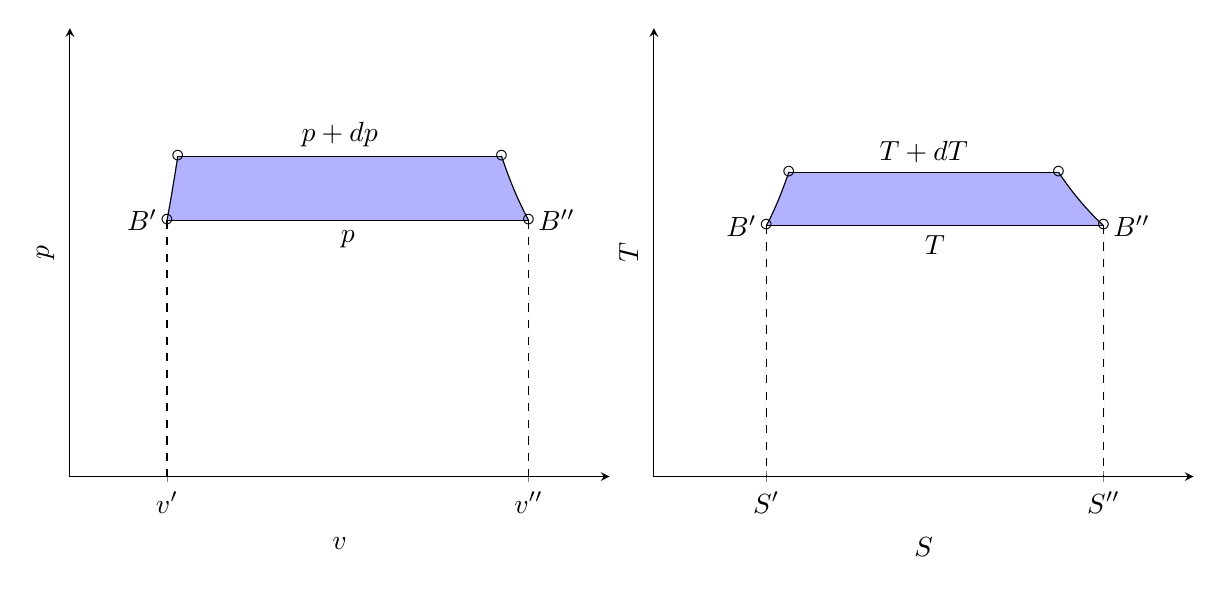
\begin{tikzpicture}
        \begin{axis}[%
    		name=plot1,
    		enlargelimits=true,
        	grid=none,
        	axis lines=left, xtick=\empty, ytick=\empty,
        	xmin = 0, xmax = 10,
        	ymin = -0.5, ymax = 10,
        	ylabel=$p$,
        	xlabel=$v$,
        	no markers,
        	xticklabels={,,},yticklabels={,,},
        	extra x ticks={1.8,8.5},
		    extra x tick labels={$v'$,$v''$}
        ]
        	\addplot+[domain=2:8,fill,blue!30] { 7 } \closedcycle;
        	\addplot+[domain=1.8:2,fill,blue!30] { 3.6111*x*x - 6.2222*x + 5 } \closedcycle;
        	\addplot+[domain=8:8.5,fill,blue!30] { 12.8333/(x-6.16667) } \closedcycle;
        	\addplot+[domain=1.8:8.5,fill,white] { 5.5 } \closedcycle;
        	
        	\addplot[domain=2:8] { 7 };
        	\addplot[domain=1.8:2] { 3.6111*x*x - 6.2222*x + 5 };
        	\addplot[domain=8:8.5] { 12.8333/(x-6.16667) };
        	\addplot[domain=1.8:8.5] { 5.5 };
        	
        	\draw (2,7) node{$\circ$};
        	\draw (8,7) node{$\circ$};
        	\draw[dashed] (1.8,5.5) node{$\circ$} node[left]{$B'$} -- (1.8,-1);
        	\draw[dashed] (8.5,5.5) node{$\circ$} node[right]{$B''$} -- (8.5,-1);
        	\draw (5,7) node[above]{$p+dp$};
        	\draw (5.15,5.5) node[below]{$p$};
    	\end{axis}
        
        \begin{axis}[%
    		name=plot2,
    		at=(plot1.right of south east), anchor=left of south west,
    		axis lines=left, xtick=\empty, ytick=\empty,
    		enlargelimits=true,
        	grid=none,
        	xmin = 0, xmax = 10,
        	ymin = -0.5, ymax = 10,
        	ylabel=$T$,
        	xlabel=$S$,
        	no markers,
        	xticklabels={,,},yticklabels={,,},
        	extra x ticks={1.5,9},
		    extra x tick labels={$S'$,$S''$}
        ]
        	\addplot+[domain=2:8,fill,blue!30] { 7 } \closedcycle;
        	\addplot+[domain=1.5:2,fill,blue!30] { (4/3)*x*x - (5/3)*x + 5 } \closedcycle;
        	\addplot+[domain=8:9,fill,blue!30] { (77/3)/(x-(13/3)) } \closedcycle;
        	\addplot+[domain=1.5:9,fill,white] { 5.5 } \closedcycle;
        	
        	\addplot[domain=2:8] { 7 };
        	\addplot[domain=1.5:2] { (4/3)*x*x - (5/3)*x + 5 };
        	\addplot[domain=8:9] { (77/3)/(x-(13/3)) };
        	\addplot[domain=1.5:9] { 5.5 };
        	
        	\draw (2,7) node{$\circ$};
        	\draw (8,7) node{$\circ$};
        	\draw[dashed] (1.5,5.5) node{$\circ$} node[left]{$B'$} -- (1.5,-2);
        	\draw[dashed] (9,5.5) node{$\circ$} node[right]{$B''$} -- (9,-2);
        	\draw (5,7) node[above]{$T+dT$};
        	\draw (5.25,5.5) node[below]{$T$};
    	\end{axis}
    \end{tikzpicture}
    \caption{Vaporisation isobare (et isotherme) d'un fluide}
    \label{fig:vaporisation}
\end{figure}

\subsection{Calculez la variation d'énergie interne, d'enthalpie et d'entropie le long de l'isotherme liquide $T_0 = \SI{273.15}{\kelvin}$ par rapport à l'état du liquide saturé à $T_0$.}
L'état de référence choisi est celui du liquide saturé à $T_0$, représenté par le point $A_0$ de la figure \ref{fig:T0ref}. Désignons par $p_0$ la pression et $v_0$ le volume massique à l'état de référence. Les symboles $U_0$, $H_0$ et $S_0$ désignent les fonctions d'état à l'état de référence choisi. Nous pouvons dès lors définir les variations par rapport au point $A$ de l'énergie interne $u_A$, de l'enthalpie $h_A$ et de l'entropie $s_A$ que nous allons calculer par les relations respectives suivantes:
\begin{equation} u_A = U_A-U_{0} \qquad h_A = H_A-H_{0} \qquad s_A = S_A-S_{0} \end{equation}
l'état $A$ étant défini par la pression $p$ et la température $T_0$ (sur la même isotherme que $A_0$). L'étude du comportement de la substance à l'état liquide autour de $T_0=\SI{273.15}{\kelvin}$, plus particulièrement en ce qui concerne les coefficients de dilatation et de compressibilité, permet d'établir une équation d'état du liquide :
\begin{equation} v = v(T,p) \end{equation}
\paragraph{Entropie} En se rappelant que l'enthalpie libre de Gibbs $G$ est une fonction d'état, telle que :
\begin{equation} dG = -SdT + vdp \end{equation}
on déduit, par le théorème de Schwarz :
\begin{equation} -\left.\fpart{S}{p}\right|_T = \left.\fpart{v}{T}\right|_p = \alpha v \qquad \text{avec} \qquad \alpha = \frac{1}{v}\left(\fpart{v}{T}\right)_p \end{equation}
ce qui permet de calculer la varation d'entropie le long de l'isotherme $T_0$. En intégrant, on trouve :
\begin{equation} s_A = S_A-S_0 = -\int_{p_0}^{p_A}\alpha vdp = -\overline{\alpha v}(p_A-p_0) \end{equation}
où $\overline{\alpha v}$ représente la valeur moyenne de $\alpha v$ sur l'intervalle $\left[p_0,p_A\right]$. Les facteurs $\alpha$ et $v$ sont très petits, de l'ordre de $10^{-3}$ chacun pour l'eau. Il est dès lors raisonnable de négliger la valeur de leur produit et de retenir :
\begin{equation} s_A \simeq 0 \end{equation}
\paragraph{Énergie interne} La variation de $U$ est donnée par :
\begin{equation} dU = TdS - pdv \simeq -pdv \end{equation}
et donc :
\begin{equation} u_A = U_A - U_0 \simeq -\overline{p}(v_0-v_A) \end{equation}
Le volume massique n'évoluant que très peu avec la pression (le coefficient de compressibilité est de l'ordre de $10^{-4}$ pour l'eau). Il est, ici aussi, raisonnable de retenir :
\begin{equation} u_A \simeq 0 \end{equation}
\paragraph{Enthalpie} Le calcul de l'enthalpie est aisé. Par $H = U + pv$, on trouve immédiatement :
\begin{equation} h_A = H_A-H_0 = v_0(p_A-p_0) \end{equation}
Il s'agit d'une petite quantité, mais pas négligeable pour autant.
\begin{figure}[p]\centering
	\tikzsetnextfilename{T0ref}
    \begin{tikzpicture}
        \begin{axis}[
        	enlargelimits=true,
        	%grid=major,
        	axis lines=left, xtick=\empty, ytick=\empty,
        	xmin = 0.3, xmax = 3.4,
        	ymin = 0.3, ymax = 1.2,
        	ylabel=$p$,
        	xlabel=$v$,
        	xticklabels={,,},yticklabels={,,},
        	extra x ticks={0.6841,1.727},
		    extra x tick style={grid=major, grid style={dashed,black}},
		    extra x tick labels={$v'$,$v''$},
		    extra y ticks={0.8119},
		    extra y tick style={grid=major, grid style={dashed,black}},
		]
			\addplot [blue] table[col sep=comma] {data/vdw9.csv};
			\addplot [blue] table[col sep=comma] {data/vdw7.csv};
			\addplot [black,thick] table[col sep=comma] {data/vdw6.csv};
			\path[name path=axis] (0.6034,0.647) -- (2.35,0.647);
			\draw (1,1) node{$\circ$} node[above]{\small$K$};
			\draw[blue] (1.3,0.647) node[above]{$T_0$};
			\draw (0.6034,0.647) node{$\bullet$} node[left]{$A_0$};
			\draw (0.58,0.8119) node{$\bullet$} node[above left]{$A$};
			\draw (0.6841,0.8119) node{$\bullet$} node[above right]{$B'$};
			\draw (1.727,0.8119) node{$\bullet$} node[above right]{$B''$};
        \end{axis}
    \end{tikzpicture}
    \caption{Diagramme ($p$,$v$) d'un fluide vaporisable}
    \label{fig:T0ref}
\end{figure}

\subsection{Calculez les valeurs d'énergie interne $u'$, d'enthalpie $h'$ et d'entropie $s'$ pour les états de liquide saturé, ainsi que les valeurs d'énergie interne $u''$, d'enthalpie $h''$ et d'entropie $s''$ pour les états de vapeur saturé.}
Nous considérons ici la transformation isobare $AB'$ de la figure \ref{fig:T0ref}. On a :
\begin{equation} h' - h_A = q_\text{éch} = \int_{273.15}^Tc_{pl}dT \end{equation}
où $q_\text{éch}$ est la chaleur d'échauffement du liquide, l'action calorifique requise pour augmenter, sous pression constante, la température du liquide de $\SI{0}{\celsius}$ jusqu'à la température de saturation $t_\text{sat}$. Le calcul de sa valeur nécessite la détermination de celle de la chaleur massique $c_{pl}$ du liquide qui varie avec la pression et la température.
On a ensuite :
\begin{equation} u' - u_A = h' - h_A - p_A(v'-v_A) \end{equation}
d'où :
\begin{align} u' &= h' - (p_Av' - p_0v_0) \\ s'-s_A = s' &= \int_{273.15}^T\frac{c_{pl}}{T}dT \end{align}
Le calcul des valeurs $u''$, $h''$ et $s''$ pour les états de vapeur saturée est immédiat :
\begin{align} h''-h' &= h_{lv} \\ s''-s' &= \frac{h''-h'}{T_\text{sat}} = \frac{h_{lv}}{T_\text{sat}} \\ u''-u' &= h_{lv} - p(v''-v') \end{align}
où $h_{lv}$ est la chaleur de vaporisation, définie à la question \ref{q:59}.
